\documentclass[conference]{IEEEtran}
\IEEEoverridecommandlockouts

\usepackage{cite}
\usepackage{amsmath,amssymb}
\usepackage{graphicx}
\usepackage{booktabs}
\usepackage{xcolor}
\usepackage[hidelinks]{hyperref}

\graphicspath{{../results/figures/}}
\newcommand{\LRTestPRAUC}{0.461}
\newcommand{\XGBTestPRAUC}{0.468}
\newcommand{\LRTestROCAUC}{0.640}
\newcommand{\XGBTestROCAUC}{0.645}
\newcommand{\RouteTestPRAUC}{0.381}
\newcommand{\PriorTestPRAUC}{0.335}
\newcommand{\LRValPRAUC}{0.297}
\newcommand{\XGBValPRAUC}{0.276}
\newcommand{\LRTestRecallThr}{0.031}
\newcommand{\XGBTestRecallThr}{0.035}
\newcommand{\LRTestPrecThr}{0.612}
\newcommand{\XGBTestPrecThr}{0.661}
\newcommand{\LRTestRecallPfifty}{0.276}
\newcommand{\XGBTestRecallPfifty}{0.292}
\newcommand{\XGBRawECE}{0.073}
\newcommand{\XGBCalECE}{0.102}
\newcommand{\XGBRollECE}{0.047}
\newcommand{\LRRawECE}{0.064}
\newcommand{\LRCalECE}{0.103}
\newcommand{\LRRollECE}{0.045}
\newcommand{\XGBMeanPredCal}{0.234}
\newcommand{\XGBRollPRAUC}{0.450}
\newcommand{\XGBRollRecallThr}{0.062}
\newcommand{\XGBRollPrecThr}{0.585}
\newcommand{\LRRollRecallThr}{0.014}
\newcommand{\LRRollPrecThr}{0.557}
\newcommand{\XGBRollWindow}{28}
\newcommand{\LRRollWindow}{28}
\newcommand{\TestRate}{0.335}
\newcommand{\ValRate}{0.178}
\newcommand{\TrainRate}{0.250}
\newcommand{\LRTrainPRAUC}{0.452}
\newcommand{\XGBTrainPRAUC}{0.526}
\newcommand{\LRTrainROCAUC}{0.710}
\newcommand{\XGBTrainROCAUC}{0.752}
\newcommand{\LRValROCAUC}{0.664}
\newcommand{\XGBValROCAUC}{0.650}
\newcommand{\LRC}{10}
\newcommand{\XGBDepth}{4}
\newcommand{\XGBMinChild}{2000}
\newcommand{\XGBLambda}{20}
\newcommand{\XGBTrees}{308}
\newcommand{\NTrain}{244{,}737}
\newcommand{\NVal}{55{,}589}
\newcommand{\NTest}{27{,}020}

\newcommand{\RSFlagged}{1{,}979}
\newcommand{\RSMoved}{133}
\newcommand{\RSEarlier}{98}
\newcommand{\RSRiskBefore}{0.571}
\newcommand{\RSRiskAfter}{0.510}
\newcommand{\RSExpBefore}{1123}
\newcommand{\RSExpAfter}{1115}
\newcommand{\RSFlaggedRate}{0.520}


\begin{document}

\title{Day-Ahead Flight Delay Risk Prediction with\\Leakage-Free Features and Calibrated Classifiers}

\author{
\IEEEauthorblockN{Atanu Adhikari, Sambhav Kumar, Nishant Ranjan Singh,\\
Sankalp M Tellur, Prince Kumar Singh}
\IEEEauthorblockA{Advanced Machine Learning Course Project --- Phase 1}
}

\maketitle

\begin{abstract}
We predict, on the night before departure, whether a flight leaving New York City
will arrive 15 or more minutes late. Using the 2013 NYC flights data
(336{,}776 departures), we build schedule, calendar, congestion and historical-delay
features that are either known from the published schedule or computed from strictly
earlier dates, and we verify this with an automated leakage test. Logistic regression
and XGBoost are tuned on October--November and tested once on December.
On December both models clearly beat a historical route-rate baseline
(PR-AUC \LRTestPRAUC{} and \XGBTestPRAUC{} vs.\ \RouteTestPRAUC{}; base rate \TestRate),
but absolute discrimination stays modest (ROC-AUC $\approx$ 0.64) because day-level
weather is not observable a day ahead. We show that a calibrator fitted on the calm
validation months under-predicts the much worse December (ECE rises from
\XGBRawECE{} to \XGBCalECE{} for XGBoost) and that a rolling 28-day Platt recalibration
fixes most of this (ECE \XGBRollECE). Finally, an offline what-if rule that moves
high-risk flights by up to two hours finds only small predicted gains, mostly from
moving flights earlier in the day.
\end{abstract}

\begin{IEEEkeywords}
flight delay prediction, gradient boosting, logistic regression, probability calibration, data leakage, temporal validation
\end{IEEEkeywords}

%=====================================================================
\section{Introduction}
Flight delays are costly for airlines and passengers; a study commissioned by the US
FAA estimated the total annual cost of delays in the United States in the tens of
billions of dollars \cite{ball2010}. A delay risk score that is available
\emph{before} the day of operation could support decisions such as adding schedule
buffer, re-timing a flight or warning passengers with tight connections.

Many published delay models use information that is only known close to or after
departure, such as the departure delay itself or observed weather, and evaluate on
random train/test splits \cite{sternberg2017review}. Both choices make the problem
easier than it is in practice. In this project we fix the decision time to the night
before the flight and enforce it strictly. Our contributions are:
\begin{itemize}
\item a leakage-free feature pipeline (schedule, calendar, congestion, smoothed
  long-run and recent delay history) with an automated test that fails if any feature
  depends on same-day or future outcomes;
\item a comparison of logistic regression (LR) and XGBoost under a chronological
  split, with PR-AUC, ROC-AUC, recall at a fixed precision and calibration;
\item an analysis of calibration under the base-rate shift between validation and test
  months, and a rolling recalibration that adapts to it;
\item an offline what-if rescheduling analysis with explicit assumptions.
\end{itemize}

%=====================================================================
\section{Literature Review}
\textbf{Delay prediction.} Sternberg et al.\ \cite{sternberg2017review} review flight
delay prediction and group the methods into statistical analysis, probabilistic models, network
representation, operational research and machine learning; they note that results are hard to compare because
studies differ in scope, delay definition and data. Rebollo and Balakrishnan
\cite{rebollo2014} predict delays on US routes with random forests, using network
delay states as features, and show that the predictive power drops as the prediction
horizon grows, which is consistent with our day-ahead setting being hard.
Choi et al.\ \cite{choi2016} combine on-time performance data with weather
observations and compare decision trees, random forests, AdaBoost and $k$-NN,
using sampling to handle class imbalance. Gui et al.\ \cite{gui2020} combine
flight, weather and ADS-B data and compare LSTM and random forest models.
Yazdi et al.\ \cite{yazdi2020} propose a deep network trained with the
Levenberg--Marquardt algorithm on US flight data. Most of these works use observed
weather or near-departure network state, which is not available at our decision time.

\textbf{Delay propagation.} Pyrgiotis et al.\ \cite{pyrgiotis2013} model how delays
propagate through an airport network via aircraft rotations. This motivates our
features on the aircraft's position in its daily rotation and on recent airport delay
levels, and it explains the strong time-of-day effect in our data.

\textbf{Models.} Gradient boosting \cite{friedman2001} fits an additive model of
regression trees by functional gradient descent; XGBoost \cite{chen2016xgboost}
adds a second-order approximation of the loss and explicit regularisation of the
tree structure. Logistic regression remains a strong baseline for tabular risk
models and is the AML baseline required by the project brief.

\textbf{Calibration.} For a risk score to be used in decisions, its probabilities
should be calibrated. Platt scaling \cite{platt1999} fits a sigmoid on the model score;
isotonic regression \cite{zadrozny2002} fits a monotone step function.
Niculescu-Mizil and Caruana \cite{niculescu2005} show that boosted trees are often
poorly calibrated and benefit from these corrections, and Guo et al.\
\cite{guo2017calibration} popularised the expected calibration error (ECE) and
reliability diagrams. When the class prior changes between training and deployment
(label shift), the posterior must be adjusted \cite{saerens2002,lipton2018};
more generally, models in non-stationary settings need to adapt to drift
\cite{gama2014}.

\textbf{Evaluation and leakage.} With imbalanced classes the precision--recall curve is
more informative than ROC \cite{saito2015}. Kaufman et al.\ \cite{kaufman2012leakage}
formalise leakage as the use of information that would not be available at prediction
time, which is the main pitfall in delay prediction.

\textbf{Gap.} Compared to prior work, we restrict ourselves to strictly day-ahead
information, verify that restriction with a test, split chronologically, and report
calibration under temporal shift rather than only ranking metrics.

%=====================================================================
\section{Dataset and Exploratory Analysis}
We use the Kaggle copy of \texttt{nycflights13} \cite{nycflights13}: all 336{,}776
domestic departures from EWR, JFK and LGA in 2013, operated by 16 carriers to 105
destinations with 4{,}043 aircraft. The data come from the BTS on-time performance
reporting \cite{bts_ontime}.

\textbf{Quality.} 8{,}255 flights were cancelled (no departure time) and 1{,}175 departed
but have no arrival delay (diverted). These 9{,}430 flights cannot be labelled, so they
are excluded as examples but kept when counting scheduled volume, since the schedule
is known in advance. 2{,}512 rows have no tail number; there are no duplicate ids.

\textbf{Target.} A flight is \emph{delayed} if \texttt{arr\_delay} $\ge 15$ minutes,
the BTS definition. 24.5\% of labelled flights are delayed. The delay distribution is
strongly right-skewed (median $-5$ minutes, maximum 1{,}272 minutes).

\textbf{Leakage.} Departure delay and arrival delay have a correlation of 0.915, so
any post-departure field (\texttt{dep\_time}, \texttt{dep\_delay}, \texttt{arr\_time},
\texttt{air\_time}) would leak the label; all are removed.

\textbf{Seasonality and split.} Fig.~\ref{fig:month} shows large month-to-month
variation, from 13.7\% delayed in September to 33.5\% in December. Our
chronological split trains on January--September, validates on October--November
(base rate \ValRate) and tests on December (\TestRate). The test month is therefore the
worst month of the year and the validation months among the calmest, a shift that
drives several of our findings.

\begin{figure}[t]
\centering
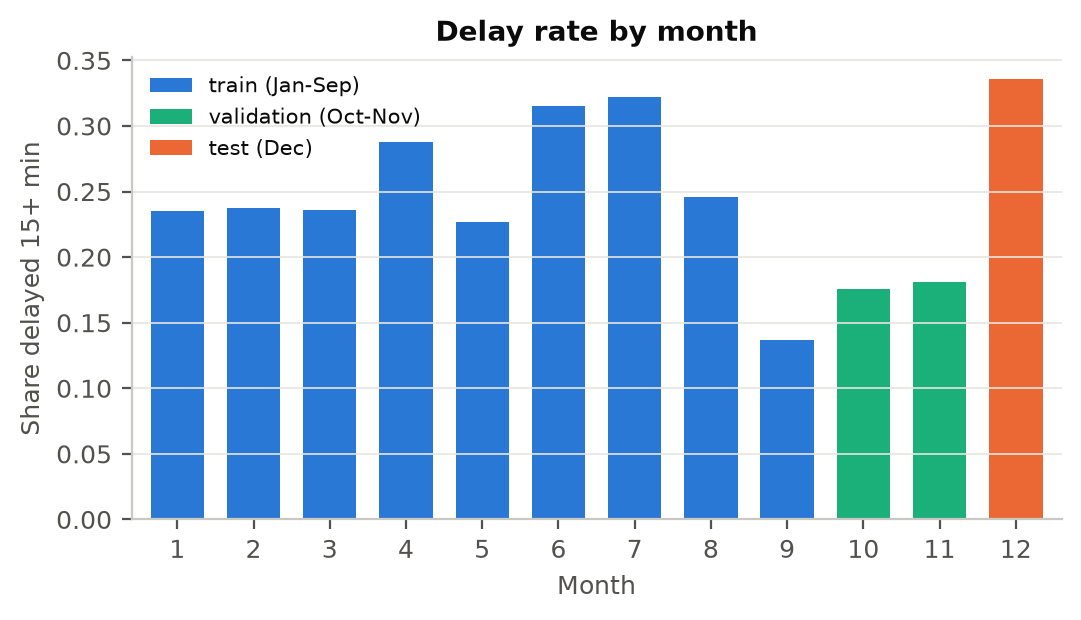
\includegraphics[width=\columnwidth]{eda_month.png}
\caption{Share of flights delayed 15+ minutes per month, coloured by split.}
\label{fig:month}
\end{figure}

\textbf{Time of day and persistence.} The delay rate rises steadily from 10.5\% for
05:00 departures to 37\% at 21:00 (Fig.~\ref{fig:eda}, left), the
signature of delay propagation. Saturday is the best day (17.5\%) and Thursday the
worst (28.5\%). The daily delay rate has a lag-1 autocorrelation of 0.40 that drops to
0.13 at lag 2 (Fig.~\ref{fig:eda}, right): disruption carries over to the next day but
fades quickly. Carriers with at least 1{,}000 flights range from about 19\% to 35\%
delayed, and many routes and flight numbers have few observations, which motivates
smoothing of historical rates.

\begin{figure*}[t]
\centering
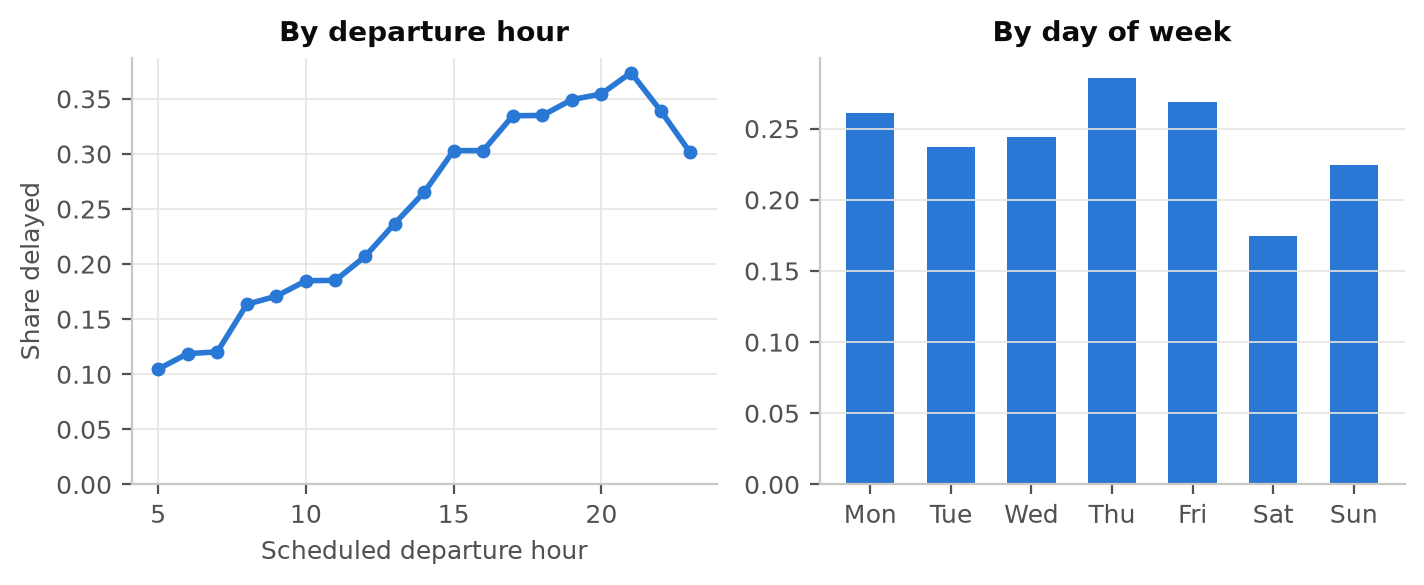
\includegraphics[width=0.49\textwidth]{eda_hour_dow.png}\hfill
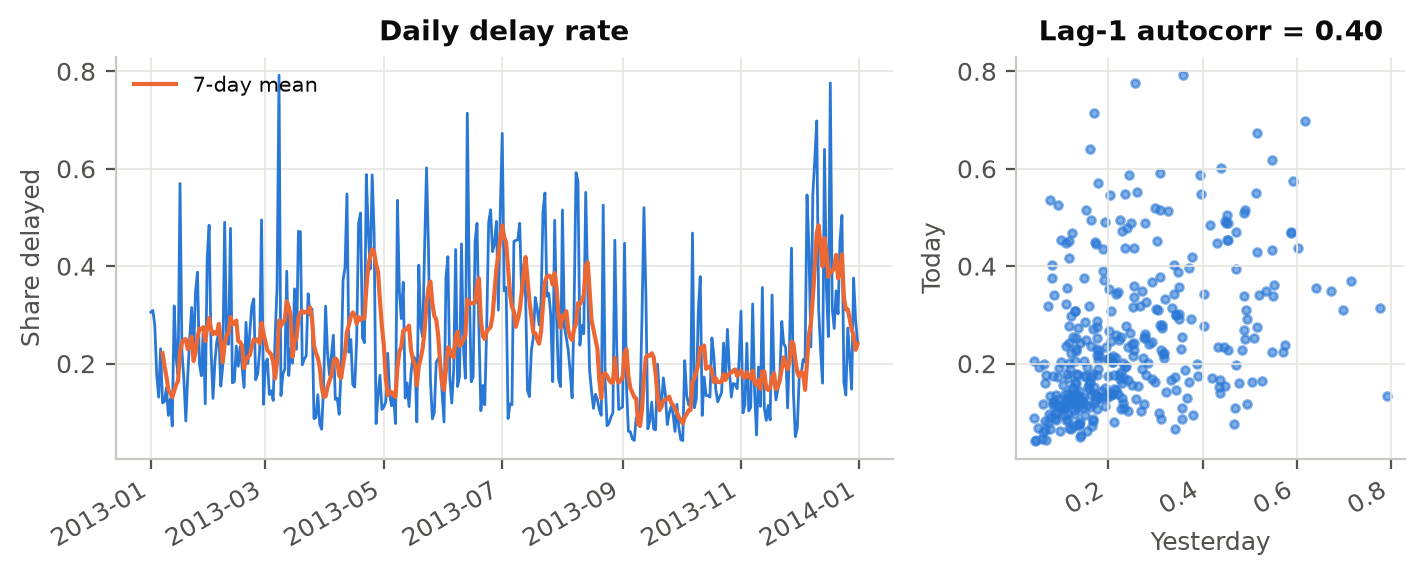
\includegraphics[width=0.49\textwidth]{eda_daily.png}
\caption{Left: delay rate by scheduled departure hour and day of week. Right: daily
delay rate over 2013 and yesterday-vs-today scatter.}
\label{fig:eda}
\end{figure*}

%=====================================================================
\section{Problem Formulation}
Let flight $i$ be scheduled on date $d_i$ with schedule attributes $s_i$ (carrier,
origin, destination, scheduled times, distance, aircraft). The decision is made at the
end of day $d_i - 1$. The information set is
\begin{equation}
\mathcal{I}_i = \{ s_j : d_j = d_i \} \cup \{ (s_j, y_j) : d_j < d_i \},
\end{equation}
i.e.\ the full schedule of the day (published in advance) plus outcomes of all earlier
days. We assume outcomes of day $d_i - 1$ are known at the decision time; a few late
evening flights land after midnight, which makes this assumption slightly optimistic.
The task is to estimate $P(y_i = 1 \mid \mathcal{I}_i)$ with $y_i = \mathbb{1}[\text{arr\_delay}_i \ge 15]$.

%=====================================================================
\section{Feature Engineering}
All 35 features (3 categorical, 32 numeric) fall into five groups (Table~\ref{tab:features}).

\begin{table}[t]
\caption{Feature groups}
\label{tab:features}
\centering
\small
\begin{tabular}{p{0.24\columnwidth}p{0.66\columnwidth}}
\toprule
Group & Features \\
\midrule
Categorical & carrier, origin, destination \\
Calendar & sin/cos of scheduled departure and arrival time of day, sin/cos of day of week, weekend flag, days to nearest US federal holiday \\
Schedule & departure hour, distance, overnight arrival flag \\
Congestion & scheduled departures per origin-day, per origin-hour, per destination-day, per carrier-day; aircraft's number of NYC departures that day and position of this leg \\
Long-run history & smoothed past delay rate per carrier, origin, destination, route, carrier-route, origin-hour, flight number, aircraft \\
Recent history & smoothed 7-day delay rate per origin, carrier, destination; previous day's system and origin delay rate, origin cancellation rate and mean arrival delay \\
\bottomrule
\end{tabular}
\end{table}

\textbf{Cyclic encoding.} Time of day $t$ (minutes) is encoded as
$(\sin 2\pi t/1440, \cos 2\pi t/1440)$ so that 23:59 and 00:00 are close.

\textbf{Past-only aggregation.} For a grouping key $g$ (e.g.\ route) let $k_g(d)$ and
$n_g(d)$ be the number of delayed and of labelled flights of $g$ on day $d$. The
history features for a flight on day $d$ use only
\begin{equation}
K_g(d) = \sum_{d' < d} k_g(d'), \qquad N_g(d) = \sum_{d' < d} n_g(d'),
\end{equation}
or the same sums restricted to $d-w \le d' < d$ for a window of $w$ days. In code this
is a cumulative (or rolling) sum over a daily table followed by a one-day shift.

\textbf{Smoothing.} Raw rates $K/N$ are noisy for rare keys. We shrink them towards the
system-wide past rate $p_0(d)$ with $m=20$ pseudo-observations,
\begin{equation}
\hat r_g(d) = \frac{K_g(d) + m\, p_0(d)}{N_g(d) + m},
\end{equation}
which is the posterior mean under a $\mathrm{Beta}(m p_0, m(1-p_0))$ prior and the
same idea as target encoding with smoothing \cite{micci2001}.

\textbf{Leakage test.} The feature notebook builds the features, then replaces
all outcomes on and after a cutoff date with random values and rebuilds them. Every
feature on or before the cutoff must be unchanged. We also checked that the test fails
when the one-day shift is removed.

\textbf{Removed features.} Day-of-year and month features were dropped: with one year of
data, October--December never appear in training, so their seasonality cannot be
learned, and in preliminary validation runs they only helped XGBoost memorise
particular training days.

%=====================================================================
\section{Methods}
\subsection{Logistic Regression}
LR models $p_i = \sigma(\mathbf{w}^\top \mathbf{x}_i + b)$ and minimises the
L2-regularised log-loss
\begin{equation}
\mathcal{L}(\mathbf{w}, b) = -\sum_i \big[y_i \log p_i + (1-y_i)\log(1-p_i)\big] + \frac{1}{2C}\lVert\mathbf{w}\rVert^2 .
\end{equation}
The objective is convex, so the solution is unique. At the optimum the gradient with
respect to $b$ vanishes, giving $\sum_i p_i = \sum_i y_i$: LR is calibrated in the large
on its training data, so its raw probabilities are anchored to the January--September
base rate (\TrainRate) rather than to the calm validation months. Numeric features are median-imputed and standardised; categoricals are
one-hot encoded (levels with fewer than 50 flights are pooled).

\subsection{XGBoost}
XGBoost \cite{chen2016xgboost} builds $F(\mathbf{x}) = \sum_k f_k(\mathbf{x})$ from
regression trees and minimises
$\sum_i \ell(y_i, F(\mathbf{x}_i)) + \sum_k \Omega(f_k)$ with
$\Omega(f) = \gamma T + \tfrac{1}{2}\lambda \lVert \mathbf{w} \rVert^2$, where $T$ is
the number of leaves and $\mathbf{w}$ the leaf values. Each new tree uses a
second-order expansion with $g_i = p_i - y_i$ and $h_i = p_i(1-p_i)$ for log-loss.
For a leaf with instance set $I_j$, $G_j = \sum_{I_j} g_i$, $H_j = \sum_{I_j} h_i$,
the optimal value is $w_j^* = -G_j / (H_j + \lambda)$ and a split gains
\begin{equation}
\frac{1}{2}\left[\frac{G_L^2}{H_L+\lambda} + \frac{G_R^2}{H_R+\lambda} - \frac{(G_L+G_R)^2}{H_L+H_R+\lambda}\right] - \gamma .
\end{equation}
The \texttt{min\_child\_weight} parameter requires $H_j$ above a threshold. Since
$h_i \le 1/4$, a value of 2000 forces at least 8{,}000 flights into every leaf, about
nine days of NYC departures. This turned out to be essential (Sec.~\ref{sec:overfit}).
Categoricals are handled natively.

\subsection{Calibration}
\emph{Platt scaling} fits $q = \sigma(a \cdot \mathrm{logit}(p) + c)$ on held-out data;
\emph{isotonic regression} fits a non-decreasing step function by pool-adjacent-violators.
Both are monotone, so ranking metrics do not change. Under pure label shift, Bayes' rule
gives $\mathrm{logit}\, q = \mathrm{logit}\, p + \log\frac{\pi_t}{1-\pi_t} - \log\frac{\pi_s}{1-\pi_s}$
for source and target priors $\pi_s, \pi_t$ \cite{saerens2002}: the intercept $c$ in
Platt scaling is exactly the term that has to follow the base rate. We therefore also
use \emph{rolling} Platt scaling, refitted every day on the previous $w$ days of
out-of-sample scores and outcomes (all available at the decision time).

\subsection{Metrics}
PR-AUC (average precision) is the headline metric \cite{saito2015}; we also report
ROC-AUC, Brier score $\frac{1}{N}\sum_i (p_i - y_i)^2$ and
$\mathrm{ECE} = \sum_{b=1}^{10} \frac{|B_b|}{N} \lvert \bar y_{B_b} - \bar p_{B_b}\rvert$
with ten equal-width bins \cite{guo2017calibration}. As an operating point we require a
precision of at least 0.5 (at least half of the flagged flights are really delayed) and
report the recall achieved.

%=====================================================================
\section{Experimental Setup}
The training, validation and test sets contain \NTrain, \NVal{} and \NTest{} labelled
flights. All choices use validation data only; December is scored once.
\begin{itemize}
\item \textbf{LR:} $C \in \{10^{-3}, \dots, 10\}$, selected $C=\LRC$.
\item \textbf{XGBoost:} learning rate 0.05, subsample and column sample 0.8, up to 3000
trees with early stopping (100 rounds) on validation PR-AUC; grid over depth
$\{3,4,6\}$, \texttt{min\_child\_weight} $\{100,500,2000\}$, $\lambda \in \{1,20\}$.
Selected: depth \XGBDepth, \texttt{min\_child\_weight} \XGBMinChild, $\lambda=\XGBLambda$,
\XGBTrees{} trees.
\item \textbf{Calibration:} Platt vs.\ isotonic chosen by fitting on October and scoring
Brier on November and vice versa; Platt won for both models and was refitted on all of
validation. The rolling window $w \in \{7, 14, 28\}$ was chosen by Brier score on
November, giving $w = \XGBRollWindow$ days for both models.
\item \textbf{Threshold:} lowest threshold with validation precision $\ge 0.5$.
\item \textbf{Baselines:} constant training base rate, and the smoothed historical route
delay rate as a score.
\end{itemize}
The code is organised as five Jupyter notebooks, one work package per team member
(see Team Contributions), and uses scikit-learn \cite{pedregosa2011}
and XGBoost; running them in order reproduces every number and figure in this report. The code,
results and this report are available at
\url{https://github.com/techatanu/Flight_Delay_Risk}.

%=====================================================================
\section{Results}
\subsection{Discrimination}
Table~\ref{tab:metrics} and Fig.~\ref{fig:prroc} summarise December performance. Both
models clearly improve on the route-history baseline. XGBoost is slightly ahead of LR
on December (PR-AUC \XGBTestPRAUC{} vs.\ \LRTestPRAUC), while LR was better on
validation (\LRValPRAUC{} vs.\ \XGBValPRAUC). The difference between the two models is
small relative to the gap between validation and test periods.

\begin{table}[t]
\caption{December test results (Platt-calibrated on Oct--Nov)}
\label{tab:metrics}
\centering
\begin{tabular}{lcccc}
\toprule
Model & PR-AUC & ROC-AUC & Brier & ECE \\
\midrule
Prior rate & 0.335 & 0.500 & 0.230 & 0.086 \\
Route history & 0.381 & 0.554 & 0.230 & 0.095 \\
LR & 0.461 & 0.640 & 0.222 & 0.103 \\
XGBoost & 0.468 & 0.645 & 0.221 & 0.102 \\
\bottomrule
\end{tabular}

\end{table}

\begin{figure*}[t]
\centering
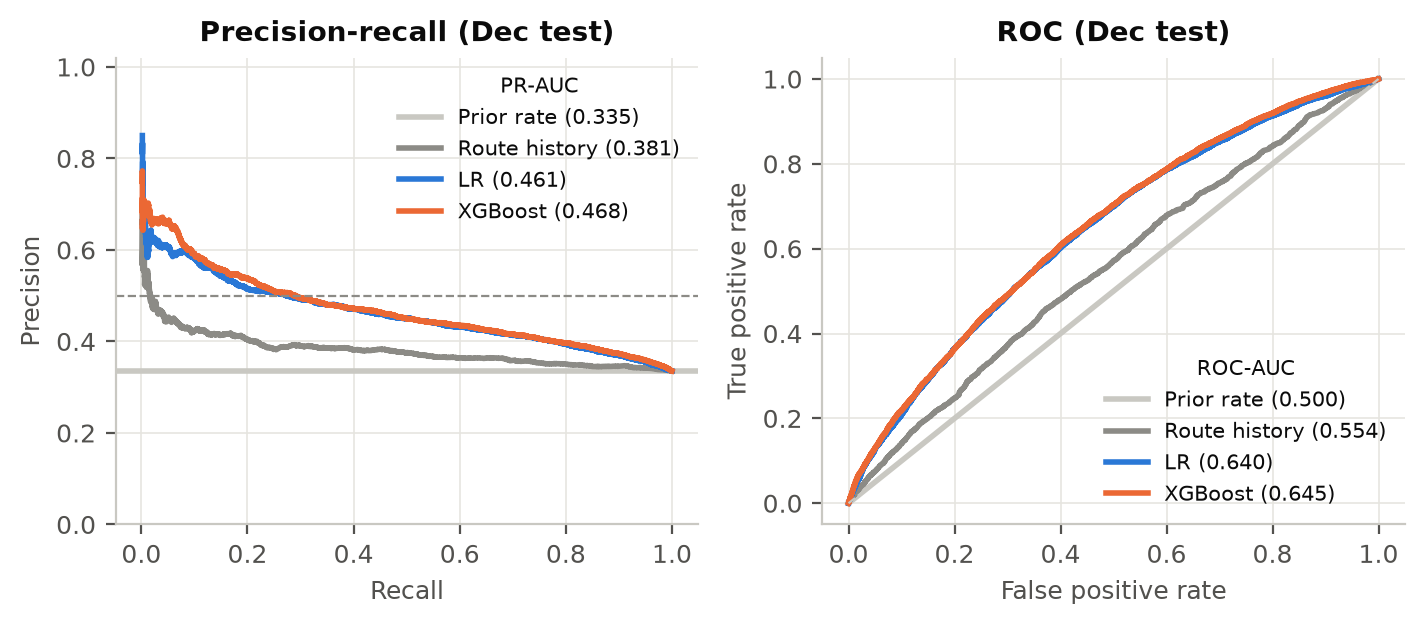
\includegraphics[width=0.85\textwidth]{pr_roc_test.png}
\caption{Precision--recall and ROC curves on the December test set. Dashed line in the
left panel: the 0.5 precision target.}
\label{fig:prroc}
\end{figure*}

\subsection{Overfitting of XGBoost}
\label{sec:overfit}
With default-sized leaves, XGBoost fits the training months far better than it
generalises: the selected model still reaches a training PR-AUC of \XGBTrainPRAUC{}
(ROC-AUC \XGBTrainROCAUC) against \XGBValPRAUC{} (\XGBValROCAUC) on validation, while LR
goes from \LRTrainPRAUC{} (\LRTrainROCAUC) to \LRValPRAUC{} (\LRValROCAUC). (PR-AUC values
are not directly comparable across periods because base rates differ, but ROC-AUC is.)
Several features are constant within a day, such as the previous-day rates, so their
combination acts as a fingerprint of the date; deep trees with small leaves use it to
memorise the weather of individual training days. The validation grid preferred the
largest \texttt{min\_child\_weight}, which forces each leaf to span many days.

\subsection{Class Imbalance}
About a quarter of training flights are delayed. We did not reweight the classes in the
main models, and Table~\ref{tab:imbalance} checks that choice: the same models
retrained with \texttt{class\_weight="balanced"} (LR) and
\texttt{scale\_pos\_weight}$\,= n_{\text{neg}}/n_{\text{pos}}$ (XGBoost), compared on raw
probabilities. Weighting leaves PR-AUC and ROC-AUC practically unchanged but inflates
every probability: the mean predicted risk rises to about 0.5 against an observed
December rate of \TestRate, and ECE more than doubles for both models. Platt scaling
could undo the shift, but then weighting would add nothing. We therefore handle the
imbalance through the metric (PR-AUC) and the precision-based threshold instead.
Oversampling such as SMOTE was not used, because synthetic flights interpolated
between different days are inconsistent with the day-level history features.

\begin{table}[t]
\caption{Effect of class weighting (raw probabilities)}
\label{tab:imbalance}
\centering
\resizebox{\columnwidth}{!}{\begin{tabular}{lccccc}
\toprule
Model & Val PR-AUC & Test PR-AUC & Test ROC-AUC & Test ECE & Mean $\hat p$ \\
\midrule
LR (unweighted) & 0.297 & 0.461 & 0.640 & 0.064 & 0.295 \\
LR, balanced class weights & 0.296 & 0.460 & 0.641 & 0.182 & 0.517 \\
XGBoost (unweighted) & 0.276 & 0.468 & 0.645 & 0.073 & 0.269 \\
XGBoost, positive weight 3.00 & 0.273 & 0.466 & 0.647 & 0.153 & 0.488 \\
\bottomrule
\end{tabular}
}
\end{table}

\subsection{Operating Point}
Table~\ref{tab:op} applies the validation threshold to December. Precision stays above
the target (\XGBTestPrecThr{} for XGBoost), but recall is only \XGBTestRecallThr: because
December is much worse than October--November, the fixed calibration under-predicts and
the threshold flags very few flights. For reference, the best recall at precision
$\ge 0.5$ that could be achieved on December (read off the test curve, so not
attainable in practice) is \XGBTestRecallPfifty{} for XGBoost and \LRTestRecallPfifty{}
for LR. With rolling calibration the XGBoost threshold recovers some recall
(\XGBRollRecallThr{} at precision \XGBRollPrecThr); for LR it does not
(\LRRollRecallThr{} at precision \LRRollPrecThr).

\begin{table}[t]
\caption{Operating point chosen on validation (precision $\ge 0.5$), applied to December}
\label{tab:op}
\centering
\small
\resizebox{\columnwidth}{!}{\begin{tabular}{lcccc}
\toprule
Model & Threshold & Flagged & Precision & Recall \\
\midrule
LR & 0.519 & 1.7\% & 0.612 & 0.031 \\
XGBoost & 0.498 & 1.8\% & 0.661 & 0.035 \\
LR (rolling cal.) & 0.648 & 0.9\% & 0.557 & 0.014 \\
XGBoost (rolling cal.) & 0.576 & 3.6\% & 0.585 & 0.062 \\
\bottomrule
\end{tabular}
}
\end{table}

\subsection{Calibration}
Table~\ref{tab:calib} and Fig.~\ref{fig:rel} compare raw, fixed and rolling Platt
probabilities on December. Fixed calibration \emph{worsens} ECE for both models (LR
\LRRawECE{} $\to$ \LRCalECE, XGBoost \XGBRawECE{} $\to$ \XGBCalECE): it learned the low
validation base rate and pulls the mean prediction down to \XGBMeanPredCal{} while the
observed rate is \TestRate. Rolling recalibration follows the shift and gives the best
ECE (\LRRollECE{} and \XGBRollECE) and the best Brier score for XGBoost. The cost is a
lower pooled PR-AUC (\XGBRollPRAUC{} for XGBoost), because each day now gets its own
monotone map, which changes the ranking \emph{across} days.

\begin{table}[t]
\caption{Calibration on December}
\label{tab:calib}
\centering
\small
\begin{tabular}{llccc}
\toprule
Model & Probabilities & Brier & ECE & Mean $\hat p$ \\
\midrule
LR & raw & 0.2159 & 0.0640 & 0.295 \\
LR & Platt (Oct-Nov) & 0.2218 & 0.1034 & 0.232 \\
LR & Platt (rolling) & 0.2168 & 0.0450 & 0.298 \\
XGBoost & raw & 0.2163 & 0.0734 & 0.269 \\
XGBoost & Platt (Oct-Nov) & 0.2205 & 0.1017 & 0.234 \\
XGBoost & Platt (rolling) & 0.2150 & 0.0474 & 0.298 \\
\bottomrule
\end{tabular}

\end{table}

\begin{figure*}[t]
\centering
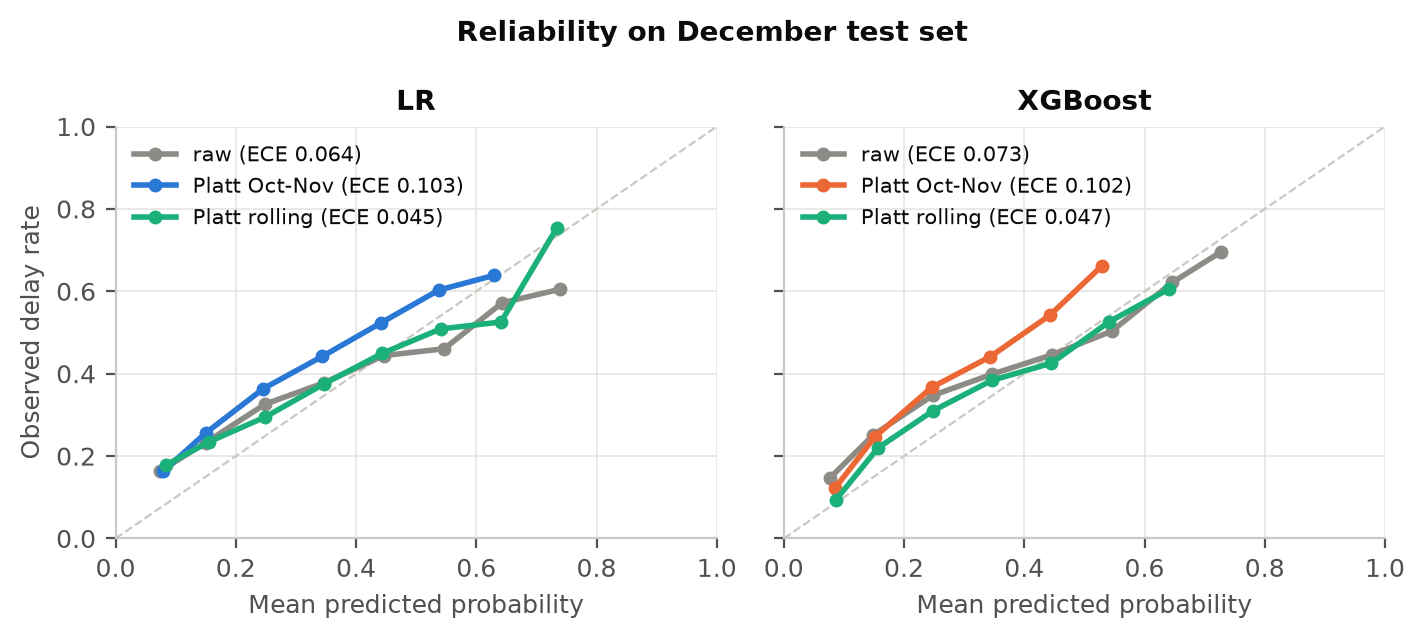
\includegraphics[width=0.85\textwidth]{reliability_test.png}
\caption{Reliability diagrams on December (bins with fewer than 50 flights omitted).}
\label{fig:rel}
\end{figure*}

\subsection{Feature Ablation and Importance}
Table~\ref{tab:ablation} and Fig.~\ref{fig:ablation} add one feature group at a time
with the selected hyperparameters. Congestion features give the largest gain on
validation. Recent-history features slightly hurt on the calm validation months but
give the largest gain on December, where disruption carries over from day to day.
This is consistent with the EDA: persistence matters on bad days and is noise on calm
ones. Permutation importance \cite{breiman2001} on validation
(Fig.~\ref{fig:imp}) ranks the scheduled daily volume at the origin, the flight
number's delay history and the departure hour highest.

\begin{table}[t]
\caption{Feature-group ablation (PR-AUC)}
\label{tab:ablation}
\centering
\small
\begin{tabular}{lcccc}
\toprule
 & \multicolumn{2}{c}{Validation} & \multicolumn{2}{c}{Test} \\
Feature set & LR & XGB & LR & XGB \\
\midrule
schedule + calendar & 0.282 & 0.288 & 0.430 & 0.436 \\
+ congestion & 0.309 & 0.297 & 0.431 & 0.424 \\
+ long-run history & 0.307 & 0.296 & 0.440 & 0.424 \\
+ recent history & 0.297 & 0.276 & 0.461 & 0.468 \\
\bottomrule
\end{tabular}

\end{table}

\begin{figure*}[t]
\centering
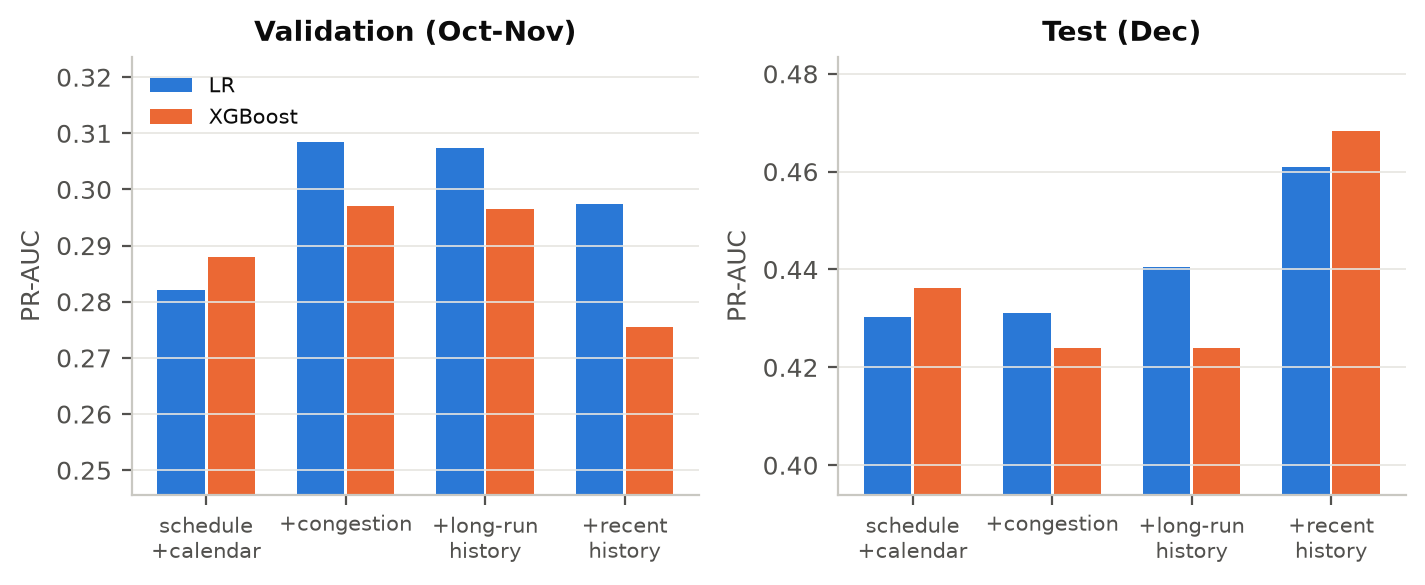
\includegraphics[width=0.85\textwidth]{ablation.png}
\caption{PR-AUC as feature groups are added (left: validation, right: test).}
\label{fig:ablation}
\end{figure*}

\begin{figure}[t]
\centering
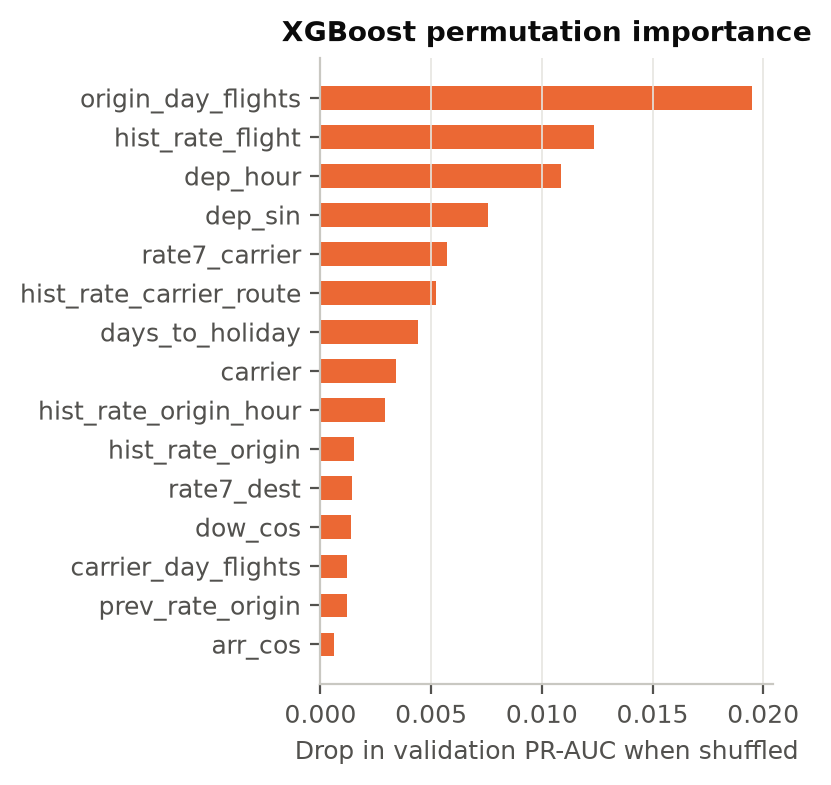
\includegraphics[width=0.85\columnwidth]{permutation_importance.png}
\caption{Top-15 features by drop in validation PR-AUC when permuted (XGBoost, 3 repeats).}
\label{fig:imp}
\end{figure}

%=====================================================================
\section{What-If Rescheduling}
\textbf{Rule.} Every December flight with predicted risk $\ge 0.5$ is offered a move of
$-2, -1, +1$ or $+2$ hours on the same day. For each candidate we recompute the
hour-dependent features (time encodings, overnight flag, origin-hour congestion
including the moved flight, origin-hour history) and score it with LR (the
best model on validation) using rolling calibration. A flight takes its best candidate
if risk drops by at least 0.05 and the target origin-hour slot has received fewer than
three moved flights; the riskiest flights choose first.

\textbf{Assumptions.} (i) The model's risk for the new slot is what the flight would face
there; the model is associational, so this is a what-if estimate, not a causal effect.
(ii) Aircraft rotations, crews, gates and passenger connections are ignored.
(iii) Flights only move into hours in which the airport already operates that day,
between 05:00 and 23:59.

\textbf{Results.} At threshold 0.5, \RSFlagged{} flights are flagged (their observed delay
rate is \RSFlaggedRate). Only \RSMoved{} have a move that clears the 0.05 gain, and
\RSEarlier{} of these move earlier; their mean risk drops from \RSRiskBefore{} to
\RSRiskAfter. Summed over all flagged flights, expected delays fall from \RSExpBefore{}
to \RSExpAfter{} (Table~\ref{tab:resched}, Fig.~\ref{fig:resched}). The model's
time-of-day profile follows the shape of the observed December profile, so the direction of
the recommendation (earlier is better) is plausible, but within $\pm 2$ hours the
predicted benefit is small. Much of the risk is attached to the day and the
route rather than the hour.

\begin{table}[t]
\caption{What-if rescheduling on December (sensitivity to the risk threshold)}
\label{tab:resched}
\centering
\small
\begin{tabular}{lccc}
\toprule
Risk threshold & 0.4 & 0.5 & 0.6 \\
\midrule
Flagged flights & 5750 & 1979 & 473 \\
Observed delay rate of flagged & 0.474 & 0.520 & 0.556 \\
Flights moved & 295 & 133 & 33 \\
Mean risk before (moved) & 0.504 & 0.571 & 0.657 \\
Mean risk after (moved) & 0.444 & 0.510 & 0.595 \\
Expected delays, flagged, before & 2796.9 & 1123.4 & 309.1 \\
Expected delays, flagged, after & 2779.1 & 1115.3 & 307.1 \\
\bottomrule
\end{tabular}

\end{table}

\begin{figure*}[t]
\centering
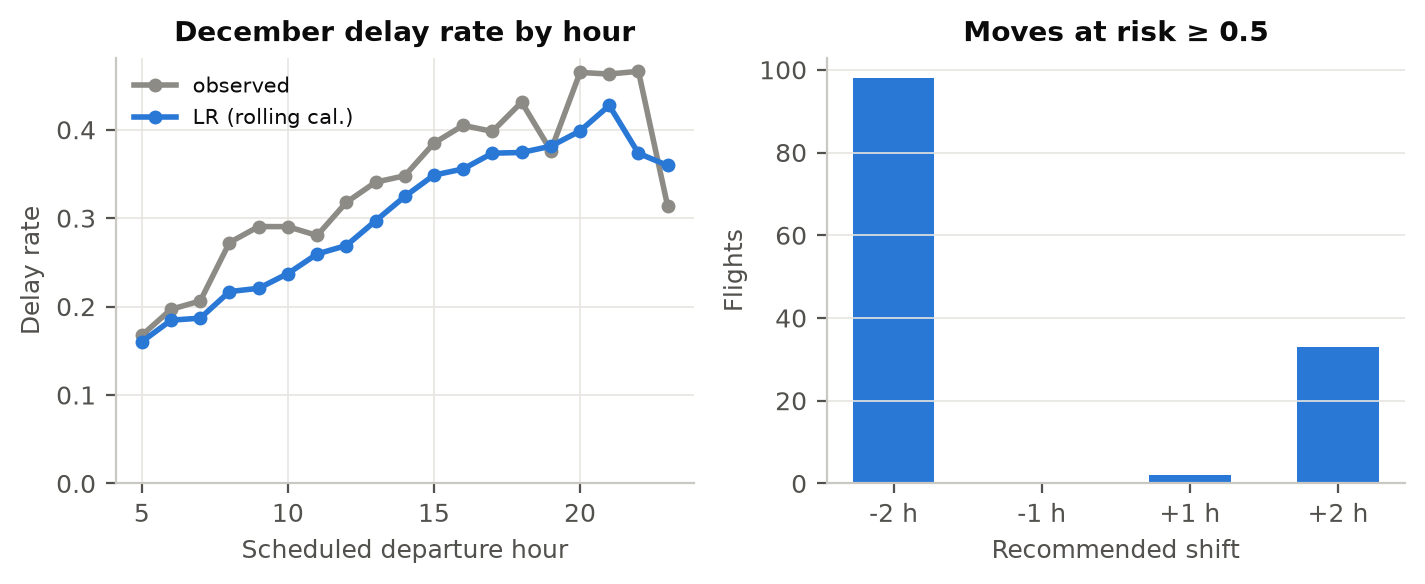
\includegraphics[width=0.85\textwidth]{reschedule.png}
\caption{Left: observed and predicted December delay rate by departure hour. Right:
recommended shifts at risk threshold 0.5.}
\label{fig:resched}
\end{figure*}

%=====================================================================
\section{Limitations}
No weather forecast is available, and the day-level weather explains much of the
variance; this caps discrimination for any day-ahead model on this data. The data
cover one year and only NYC departures, so inbound legs of an aircraft's rotation are
invisible, and seasonal effects for the test months cannot be learned. Cancelled and
diverted flights are dropped; they cluster on the worst days, so the labelled data
slightly understate disruption. The previous-day outcomes are assumed known at the
decision time. The rescheduling analysis is associational and ignores operational
constraints.

%=====================================================================
\section{Conclusion}
A strictly day-ahead delay model on the 2013 NYC flights reaches a December PR-AUC of
about 0.46--0.47 against a base rate of \TestRate, with LR and XGBoost close to each
other once XGBoost is regularised to stop memorising training days. Calibration is the
part that breaks under temporal shift: a calibrator fitted on calm months
under-predicts a bad month, and a rolling recalibration based only on past outcomes
largely repairs it. A what-if rescheduling rule finds that moving high-risk flights
earlier is the only consistent recommendation, with small predicted gains. Phase~2
will compare these models with a compact MLP that learns embeddings for carrier,
origin and destination on the same split and features.

\section*{Team Contributions}
The project was divided into five work packages, one per notebook, and the notebooks
pass their outputs to one another in order.
\begin{itemize}
\item \textbf{Atanu Adhikari} (exploratory data analysis). Audited data quality (cancelled and diverted flights, missing tail
numbers, duplicate ids), fixed the delay target and identified the post-departure
columns that must be excluded, and analysed seasonality, time of day, day of week,
carriers, routes and day-to-day persistence. This work underlies the Dataset and
Exploratory Analysis section, including the base-rate differences between the
training, validation and test months. Notebook: \texttt{01\_eda}.

\item \textbf{Sambhav Kumar} (feature engineering). Built the 35 schedule, calendar, congestion and
history features, including the past-only aggregation, the Beta-prior smoothing and the
cyclic time encodings, and wrote the leakage test that rebuilds the features after
corrupting all outcomes from a cutoff date, together with the check that a deliberately
leaky version is detected. This work underlies the Problem Formulation and Feature
Engineering sections. Notebook: \texttt{02\_feature\_engineering}.

\item \textbf{Nishant Ranjan Singh} (model training). Tuned logistic regression and XGBoost, diagnosed the
overfitting of XGBoost on training days, chose the calibration method (Platt versus
isotonic) and the rolling-calibration window on validation data, ran the class-weighting
experiment and the feature-group ablation, and saved the trained models. This work
underlies the Methods and Experimental Setup sections and the Overfitting and Class
Imbalance results. Notebook: \texttt{03\_model\_training}.

\item \textbf{Sankalp M Tellur} (evaluation and calibration). Scored all models on the December test set
(PR-AUC, ROC-AUC, Brier score, ECE), produced the precision--recall, ROC and reliability
plots, set the operating point from the validation threshold, computed permutation
importance, and generated the LaTeX tables and number macros that this report reads.
This work underlies the Discrimination, Operating Point, Calibration and Feature
Ablation and Importance results. Notebook: \texttt{04\_evaluation\_calibration}.

\item \textbf{Prince Kumar Singh} (rescheduling). Designed and implemented the what-if rescheduling analysis:
candidate moves of $\pm 1$ and $\pm 2$ hours with recomputed hour-dependent features,
the gain and slot-capacity rules, the stated assumptions, and the sensitivity to the
risk threshold. This work underlies the What-If Rescheduling section.
Notebook: \texttt{05\_rescheduling}.
\end{itemize}

\bibliographystyle{IEEEtran}
\bibliography{refs}

\end{document}